

\documentclass[conference]{IEEEtran}
% \usepackage[hmargin=.75in,vmargin=1in]{geometry}
% % *** SPECIALIZED LIST PACKAGES ***
\usepackage[american]{babel}
\usepackage[T1]{fontenc}
\usepackage{times}
\usepackage{caption}
\usepackage{subfig}
% \usepackage{algorithm}
% \usepackage{algorithmic}
\usepackage{textcomp}
\usepackage{epsfig,graphicx, graphics}
\usepackage{xcolor}
\usepackage{amsfonts,amsmath,amssymb}
\usepackage{fixltx2e} % Fixing numbering problem when using figure/table* 
\usepackage{booktabs}
\makeatletter
\let\@currsize\normalsize
\makeatother
\usepackage{setspace}
\usepackage[ruled,vlined]{algorithm2e}
% \usepackage{algorithmic}
\usepackage{soul} %corrections highlighting
\usepackage{array,multirow}
\usepackage{filecontents}
\usepackage{url}
\usepackage{cite}


% new command for editing
%\newcommand{\ts}[1]{{{\color{orange} \textbf{(Tianshu: #1)}}}}
%\newcommand{\tsc}[1]{{{\color{orange} \textbf{#1}}}}


\begin{document}
% make the title area
\title{Future Power Grid with Distributed Energy Resources:
Emerging Concerns and Mitigations}

 \author{\IEEEauthorblockN{DE-OE0000826 Technical Report} 
Authors: 


 }
\maketitle


\begin{abstract}
Availability, integrity and confidentiality are major components of energy system cyber security for buildings and power grid integration, and for secure and reliable energy distribution. As the integration of buildings and power grid evolves to accommodate distributed energy and transactive control, the amount and speed at which data is exchanged increases significantly along with expanding cyber attack surface.  Additionally, sophisticated and targeted cyber-attacks are increasing and becoming more difficult to detect and defend. At the same time, power grid utilities are moving towards a smarter grid using new technologies such as, smart meters, real-time pricing, demand side flexibility, and Distributed Energy Resources (DER). These advanced smart grid technologies are designed and deployed to improve the operations and the efficacy of the electrical grid; but there is a cost with these technologies: increased system exposure and expanded attack surface. These exposures provide new cyber security vulnerabilities that have the potential to be exploited by attackers. 

A significant challenge in energy system cyber security is the current inability to detect cyber-physical attacks targeting and originating from grid-edge systems. Cyber grid defenders have yet to design algorithms and other detection capabilities that can be used to distinguish between normal operations, cyber-attacks, and other exceptional circumstances. In this project, we propose to create  INGRESS (Integration of Green Renewable Energy Sources Securely with the Buildings and the Electric Power), a cybersecurity platform specifically designed to detect and thwart sophisticated attacks and assist utilities in supporting cyber and energy resiliency objectives. Planned to use the outcomes of the DOE-funded VOLTTRON project, INGRESS will be deployed along side legacy systems and within emerging energy system environments and will construct  models of equipment that it protects and automatically secure communications with other systems and utilities. 

This report focuses on the INGRESS system model, threat and adversary model and also potential impacts of attack to the electric power systems. 
\end{abstract}


\section{Introduction}

The complex interdependencies between the electric power grid and other critical infrastructure sectors - oil and natural gas, water, health, transportation, telecommunications and financial services - makes electric grid protection critical for our nation's economic and national security.  Recent reports depict an energy sector under constant targeted and advanced cyber-attacks that have the potential to disrupt critical systems within the electrical grid that could result in the loss of human life.  Malware such as Stuxnet, BlackEnergy, Havex  \cite{BlackEnergy:2016,Havex:2014,Sandworm:2014} are designed to attack industrial control systems found in critical infrastructure such as Supervisory Control and Data Acquisition (SCADA) systems. The threats, whether targeted or opportunistic, from criminal groups, hackers, disgruntled employees, nation states and terrorists, against critical infrastructure are evolving and growing (see incidents reported by the Industrial Control Systems Cyber Emergency Response Team (ICS CERT)~\cite{ICS-CERT:2016}). 

Since 2004, the U.S. Department of Energy (DOE) has lead strategic road mapping activities to address cyber security threats and improvements to the cyber resilience of the energy sector.  The energy sector has made significant strides in protecting the critical cyber assets at power generation and bulk power facilities through the development and enforcement of standards such as Critical Infrastructure Protection (CIP) by the North American Electric Reliability Corporation (NERC). Current power systems have advanced from a macro utility-centric model to a distributed nature that is driven by new schemes such as smart metering, real-time pricing, managing demand side flexibility and distributed renewable energy resources. These new technologies are designed to improve the operations of the electrical grid and the efficiencies of the associated markets, but they also increase system exposure, providing entry points for threat actors to disrupt grid operations.  Examples include an attacker who takes control of several smart meters and then commands them to simultaneously turn off and on, causing grid frequency variation significant enough to drive a blackout~\cite{Smartgridawareness:2015} or, an attacker who alters data at the smart meter leading to billing and trending inaccuracies~\cite{Costache:CND2011}. 

The rise of distributed energy resources (DERs - flexible loads, distributed generation, energy storage, and electric vehicles) fuel our concerns about safety, reliability and resiliency of power grids against both cyber and physical attacks from the edge. This is mainly attributed to multiple factors~\cite{Rasche:IGCTD2015},\cite{Lee:NESCOR2013}. DERs are typically deployed at homes, commercial facilities, and industrial sites. The sheer number of DER-capable assets installed in the customer sites makes direct control of DERs difficult for utilities. Locally, DERs manage generation and storage activities autonomously, based on local conditions, pre-established settings, and DER owner preferences. Utilities interact with the DER systems through owners, commercial retail energy providers, or other third party aggregators. These indirect communications can prevent utilities from implementing or enforcing necessary policies, procedures and technical controls to securely interact with grid-edge systems. DER systems located at customer sites may not be physically secured, which can make the DERs vulnerable to cyber or direct physical attacks. The owners of the systems often lack adequate cyber-security expertise and training to securely deploy, manage and control these systems. Utility-owned smart meter customers are permitted to interact with the DER systems so that direct interfaces with the DER systems may be utilized. This can cause illicit or malicious purposes where self-interested consumers manipulate their energy usage data to under-report energy consumption. Utilities typically do not have sufficient visibility into the secondary distribution and end-use levels at individual residential and commercial buildings or major DER installations. Such limited visibility may be utilized by an attacker to launch attacks on the grid through the end-user devices such as compromised smart meters, HVAC systems or renewable energy sources. A compromise on residential air conditioners that exploits the remote shut-off functionality can cause disturbances and imbalances in the grid and have the potential to cause a disruption in energy service~\cite{howtohack:2016}. 

To detect targeted cyber-attacks and achieve attack resiliency, continuous monitoring of  DERs and the DER interactions with the electrical grid in real-time is required.  The difficulty of designing such a detection scheme arises from the difficulty in tracking and extracting those inherent ``ever-changing hard-to-predict" uncertainties present in these new technologies. For example, with the distributed generation, power that used to flow in one direction, from central power plants to customers, will be flowing back from customers to the distribution grid thereby creating a reverse power flow. An adversary can inadvertently create a larger reverse power flow by attacking multiple solar systems causinng larger voltage fluctuations.  Evidences show that the integration of Distributed Generation even on a small scale without appropriate monitoring and controls could destabilize the local grid and create outages and reliability problems for local customers. Such uncertainties with no doubt can be also leveraged by an adversary to execute attacks without being detected.  

A handful of efforts have been proposed for various analyses in the power system such as distributed state estimation, topology error identification, malicious data detection etc. There are almost no techniques currently available to detect cyber-physical attacks emerging from the grid-edge devices that can have the potential to destabilize the local grid and create outages.  This paper outlines various cyber-physical attacks that can be launched from grid-edge systems and  presents INGRESS as an advanced attack detection platform deployable for both legacy and emerging behind-the-meter DER.  INGRESS is a hierarchical distributed agent based framework developed on top of VOLTTRON, and relies on the development of behavioral models of grid-edge devices in an automated and non-intrusive manner. INGRESS harnesses both data-driven and model-based techniques fusing multiple sources of information that capture the conditions of DERs and  the interconnected power grid where DERs are being integrated.  The collected information includes the data streams obtained from high-fidelity micro Phasor Measurement Units ($\mu$PMUs), DER load profiles (active and reactive power) and its operating states etc. Correlating these multiple sources of information enables INGRESS to detect attacks in the presence of uncertainties. A high level overview of the INGRESS framework is presented in Figure~\ref{ingress}.
\begin{figure}[h!]
	\centering
	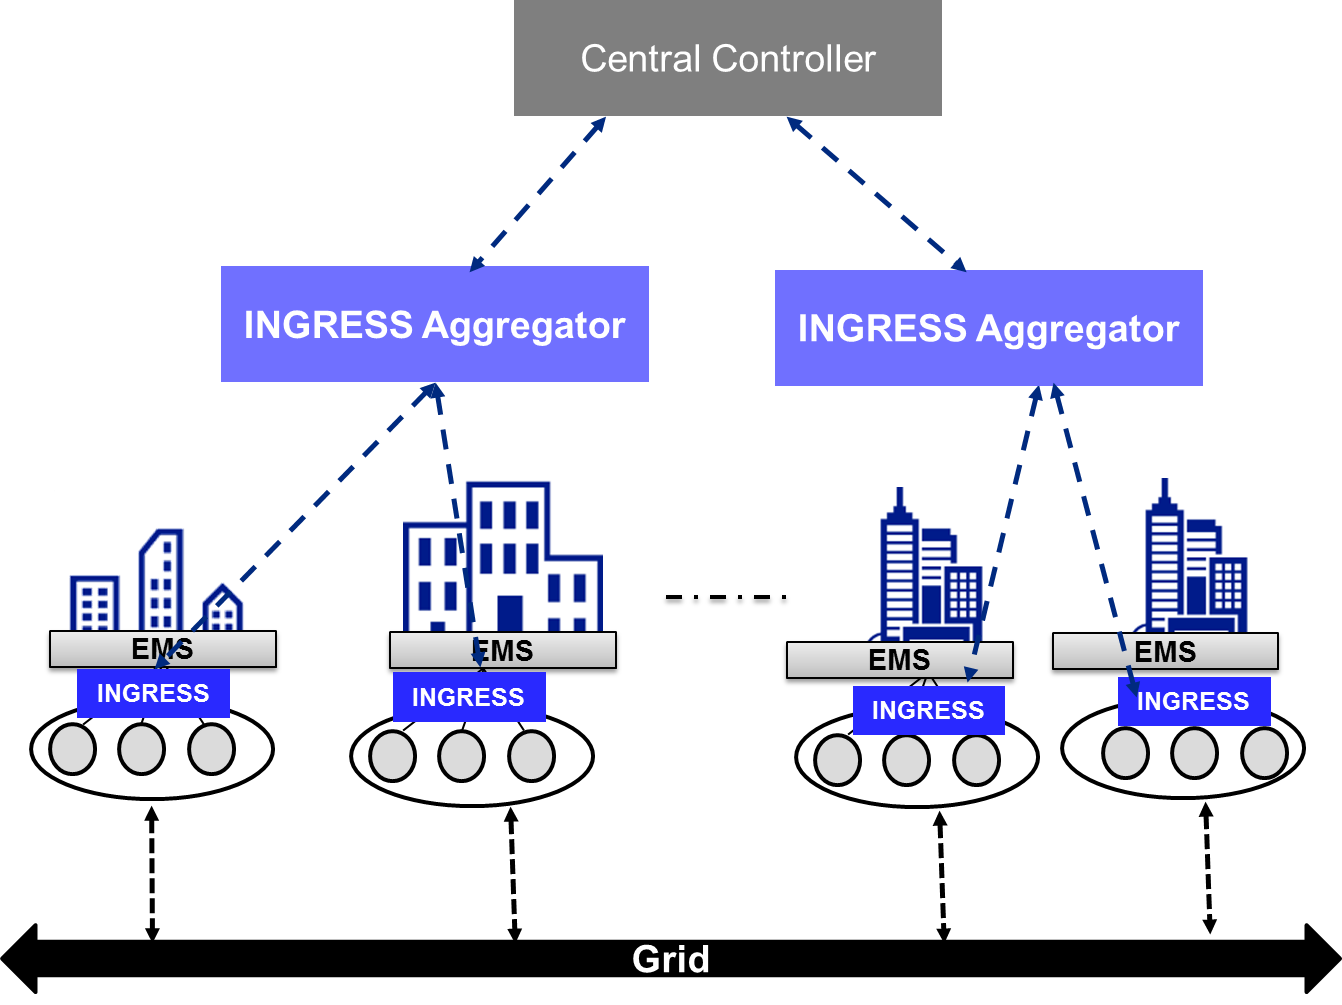
\includegraphics[width=\linewidth]{figures/ingress1.png}
	\caption{High level overview of the INGRESS framework}
	\label{ingress}
\end{figure} 
 
The remainder of the paper is organized as follows. Section~\ref{sec:system_model} presents baseline defense and security assumptions made and then our models of the power distribution system integrated with DERs and various types of attacks. Section~\ref{sec:ingress} presents a high level overview of our INGRESS framework and the various sources of information used. Section~\ref{sec:conclusion} concludes this paper.


\section{System and Adversary Model}
\label{sec:system_model}

\subsection{Baseline Defense and Security Assumptions}
Cybersecurity research community has had little success in modeling complex, evolving, non-linear cyber threats. The U.S. power grid is a complex system of systems which necessitates a narrow focus when modeling systems and adversary attacks. To help narrow the focus of this effort, this study will consider a complex, Stuxnet - like cyber attacks, where the DER is completely under the control of the attacker. Moreover, we will use the  Industrial Control System (ICS) Cyber Kill Chain (see \cite{Kushner:2013}, \cite{LeeAssante:2015}) conceptual attack frame work to better understand an attack campaign for DERs. With the increased digitization and networking of electricity infrastructure, it becomes increasingly difficult to keep adversaries out of all systems and networks. For that reason, it is important to move towards detection and resilience so even when an adversary gains access,  utilities continue to safely deliver power. 

Generally, the objective of the threat actor can be classified into three:  (a) Loss of view and control; (b) Denial of view, control, and safety; and (c) Manipulation of view, control, sensors and safety. Lee and Assante \cite{LeeAssante:2015} list the attacker objectives in the  sequence of increasing adversary sophistication. That is, manipulation is more advanced than denial, which is more advanced than loss. In considering this exploration of these objectives, it is important to note that impact and consequences vary significantly with respect to objectives. While IT penetration can lead to lateral movement and eventual escalation of privilege and damage to business goals, exploitation of operational technology (OT) may cause potential physical damage and loss of life. Impact is beyond the scope of this paper.

\subsection{Building-to-Grid Architecture and Topology Assumption}
There is not one representative structure of a typical buildings to grid (B2G) network. To increase the validity of system and adversary model as it relates to understanding the layout and structure of a typical OT network, we will leverage the Purdue Reference Model to highlight the architectural level at which the OT network and system was impacted, and the ICS Cyber Kill Chain will highlight the typical methodology of the adversary. 

\begin{figure}[h!]
	\centering
	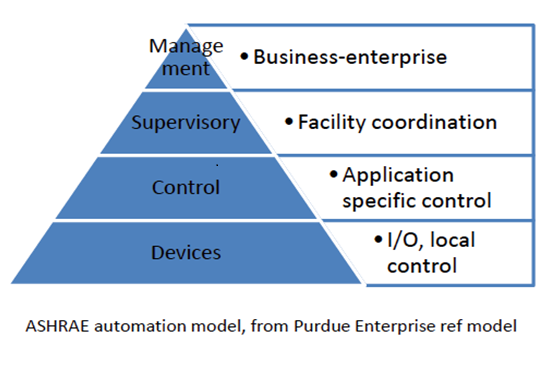
\includegraphics[width=\linewidth]{figures/prm.png}
	\caption{Purdue Reference Model}
	\label{purdue}
\end{figure} 

The following illustration highlights the different stages of a sophisticated Stuxnet attack, for e.g., how the attack targets different layers of the Purdue Reference Model (e.g., from the management to the device layer) and represents a real scenario of a completed ICS Cyber Kill Chain against a target. Stuxnet was a 500-kilobyte computer worm that contained 3 unique zero day exploits that infected 14 industrial sites in Iran, including a uranium-enrichment plant. 
For this study, we assume the following high level scenario in the context of buildings to grid deployment of DERs: For the first phase, we assume attacker compromising the servers running vulnerable operating systems or softwares and networks positioned in and accessible from the main control room.  For the second phase, a Stuxnet-type attack against  ICS software (ie. Siemens Step7 software in the case of Stuxnet) which is also and used to program industrial control systems that operate DERs is launched. In phase 3 of the attack, the DER controllers are compromised providing attackers with root access to the device.  
\begin{figure}[h!]
	\centering
	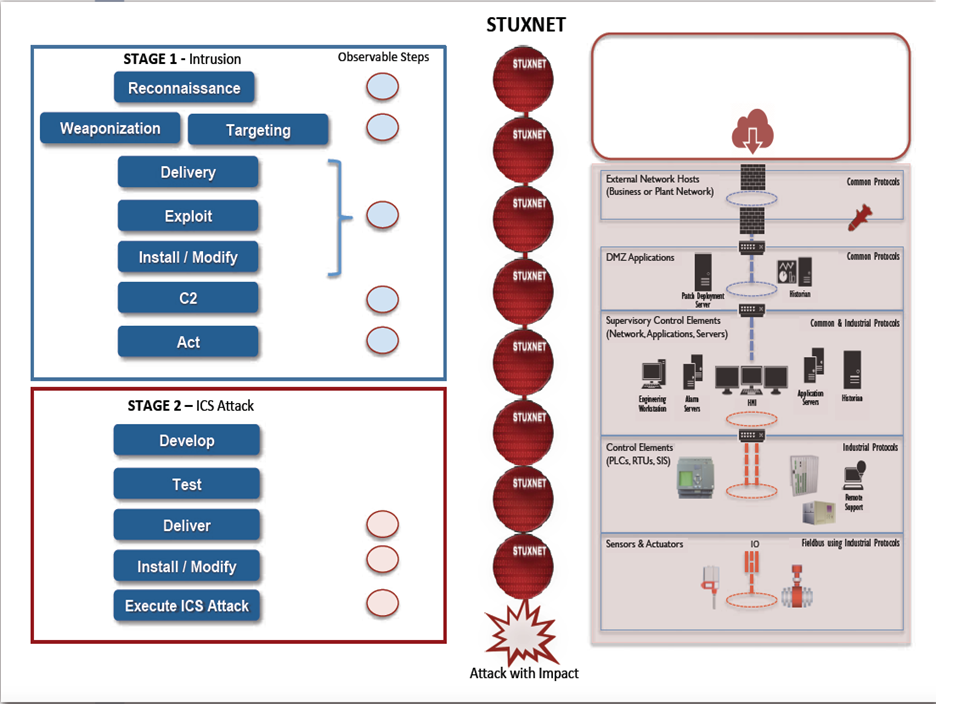
\includegraphics[width=\linewidth]{figures/stuxnet.png}
	\caption{Industrial Control System (ICS) Cyber Kill Chain}
	\label{ics}
\end{figure} 
While Stuxnet, Havex, Flame, Black Energy and sophisticated cyber payloads are challenging to defend against, it is important to note that a number of vulnerabilities are attributed to the lack of basic cybersecurity policies and procedures. The following are common system level vulnerabilities found in a converged IT/OT environment found in many smart buildings. It is especially important to explore these vulnerabilities in the context of DER implementation as buildings to grid communications are increasingly interconnected.  We acknowledge that there is no single typical building network topology or system, but the following are illustrative findings based on a number of PNNL led buildings-cyber assessments. 

\begin{figure}[h!]
	\centering
	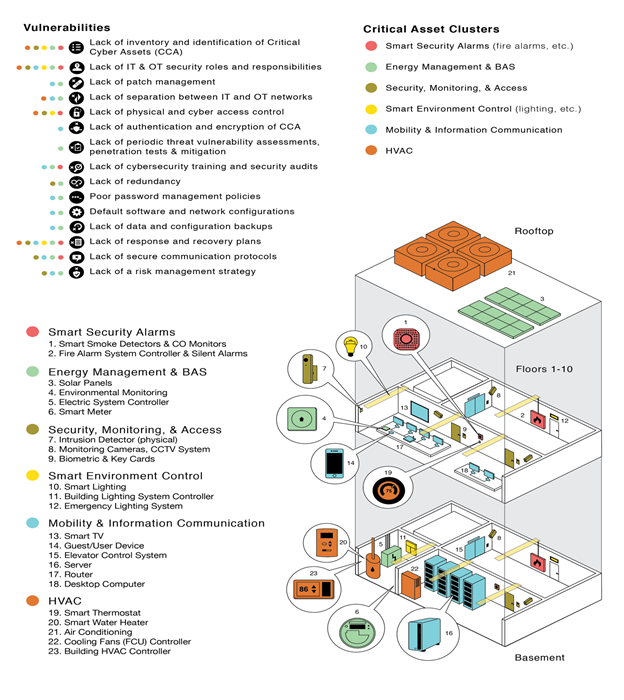
\includegraphics[width=1.1\linewidth]{figures/buildingattacks.png}
	\caption{Building cyber assessments}
	\label{battacks}
\end{figure} 

\textbf{Note:} Specifically, an attacker has multiple pathways to compromise the end system (e.g., via exploiting vulnerable servers, software, networks, web services, authorization and authentication schemes, communication protocols etc.) and defending all these pathways are challenging. The ultimate goal of the attacker is to take control of these devices to create impact on normal grid operations. This indeed motivates the design of INGRESS which will reside along with the edge device, uses multiple sources of information to learn the normal behavior of DER and detects malicious device behaviors and report the observations to higher layers (supervisory controller or central controller). The information reported will include (i) the type of affected
DER resources, (ii) estimated malicious action (e.g. voltage-frequency violations, power injection-absorption violation), and (iii) confidence level of detection with estimated severity.

\subsection{Purdue Reference based INGRESS System model} 
Figure \ref{system} provides a graphical overview of our system model, created in reference to the Purdue reference model. We assume a group of buildings connected to the distribution feeder. Each building consists of a Building or Home Energy Management System (collectively referred to as EMS in this paper) that manages and control various distributed energy resources such as demand responsive electric loads (e.g., HVAC, Electric Vehicles (EVs) and appliances) and residential solar generation. EMS (similar to supervisory under Purdue Reference Model) will be a server running Windows or Linux based OS and also embedded with web based services to interact with the external world (e.g., the management system). Each DER has local (on-board) sensors and actuators with some limited built-in intelligence that gives the DER the
ability to run autonomously for periods of time when no communication exists with the supervisory controller at the EMS. The local sensors in each DER transmit their data to the local/supervisory controller 
where the necessary control calculations are carried out and the control commands are sent back to each
DER. The EMS is further connected to the Internet for gathering external information (e.g., weather, real-time market prices) and can also respond to external data feeds, prices and demand requests from utilities/central controller and human commands by controlling the DER operation. 
\begin{figure}[h!]
	\centering
	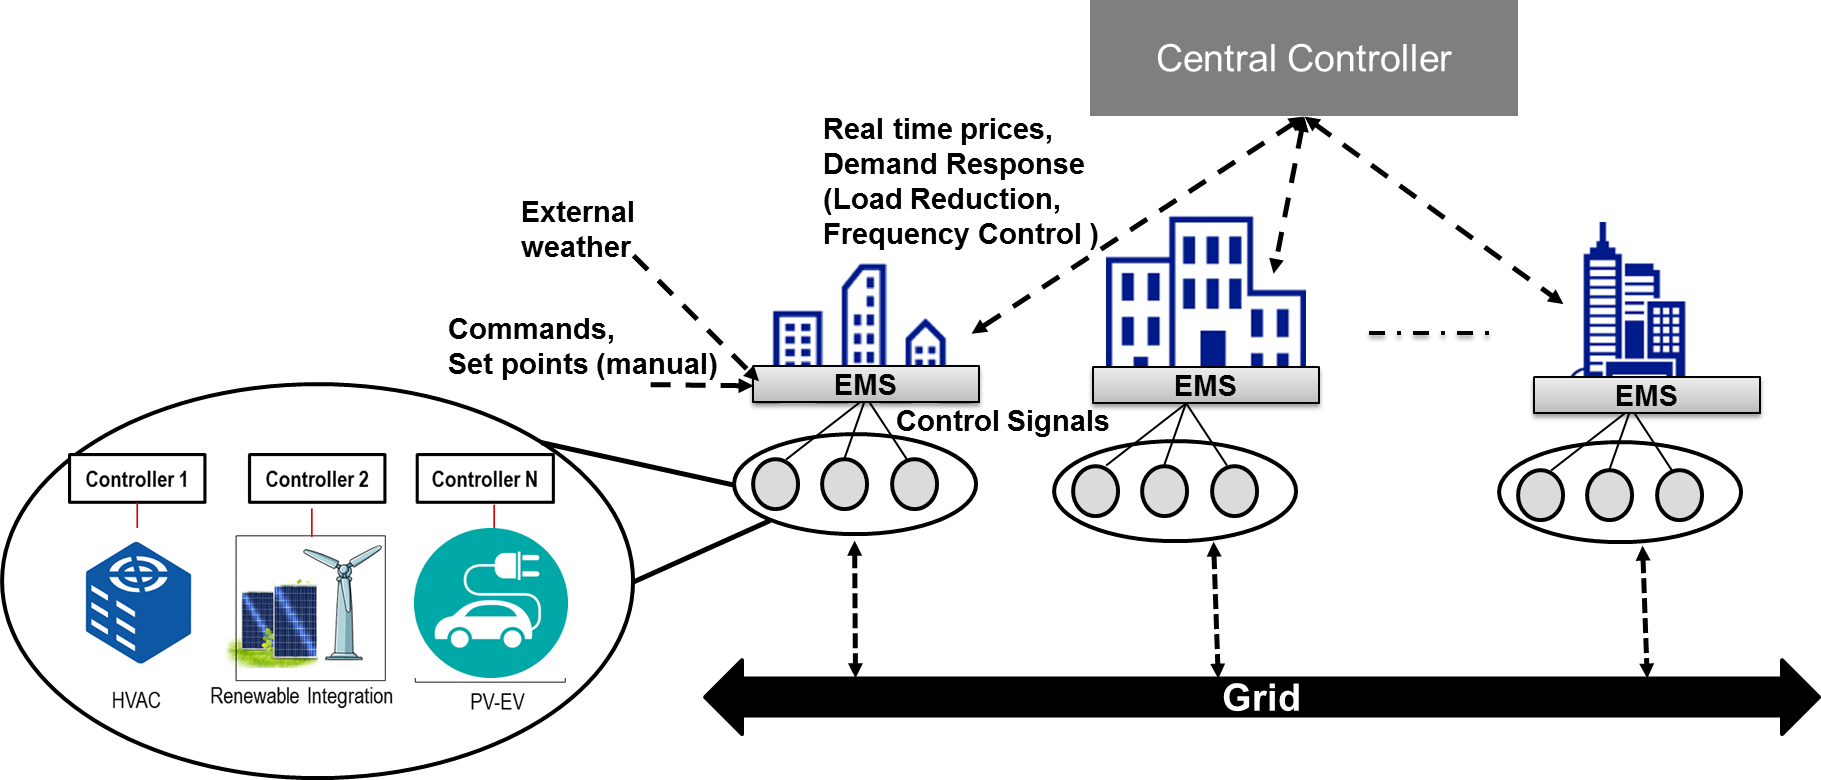
\includegraphics[width=1\linewidth]{figures/system.png}
	\caption{System Model}
	\label{system}
\end{figure}

\subsection{Adversary model} We define a malicious attacker as an adversary whose goal is to cause local outages, equipment damages or grid instabilities by controlling the DERs connected to a distribution network via the interfaces (a), (b) and (c) shown in Figure \ref{ad}. Key targets of the attacker include DER controllers and their interactions with the EMS, EMS and the interactions of EMS with the external world. An attack against DER could target a number of devices, EMS
communication networks owned by either the utility or the DER owner. The objective of the attacker is exploit these key targets to either send malicious inputs to the DERs (e.g., control requests or parameters) or completely comprises the DER controller software and the algorithms residing within it to cause voltage-frequency violations. The attack is assumed to be launched through the following means: (a) By exploiting the communication interface between the central controller and the EMS via spoofing or man-in-the-middle attacks (for e.g., by exploiting the weaknesses in the secure communication protocol). Such an attack can lead to high impact as an attacker could control multiple distributed resources that belongs to multiple distribution feeder networks; (b) By tampering the inputs to the EMS (e.g., human commands, prices, demand requests) or by compromising the EMS operating systems or software or the HMI (Human Machine Interface) and (c) By corrupting the local DER controller or the inputs to the DER  (e.g.. similar to Stuxnet attack). The impact of an attack depends on the number of devices compromised, the location of the devices (e.g., close to the substation or away from the substation), the condition, configuration and characteristics of the distribution feeder etc.  
%
\begin{figure}
	\centering
	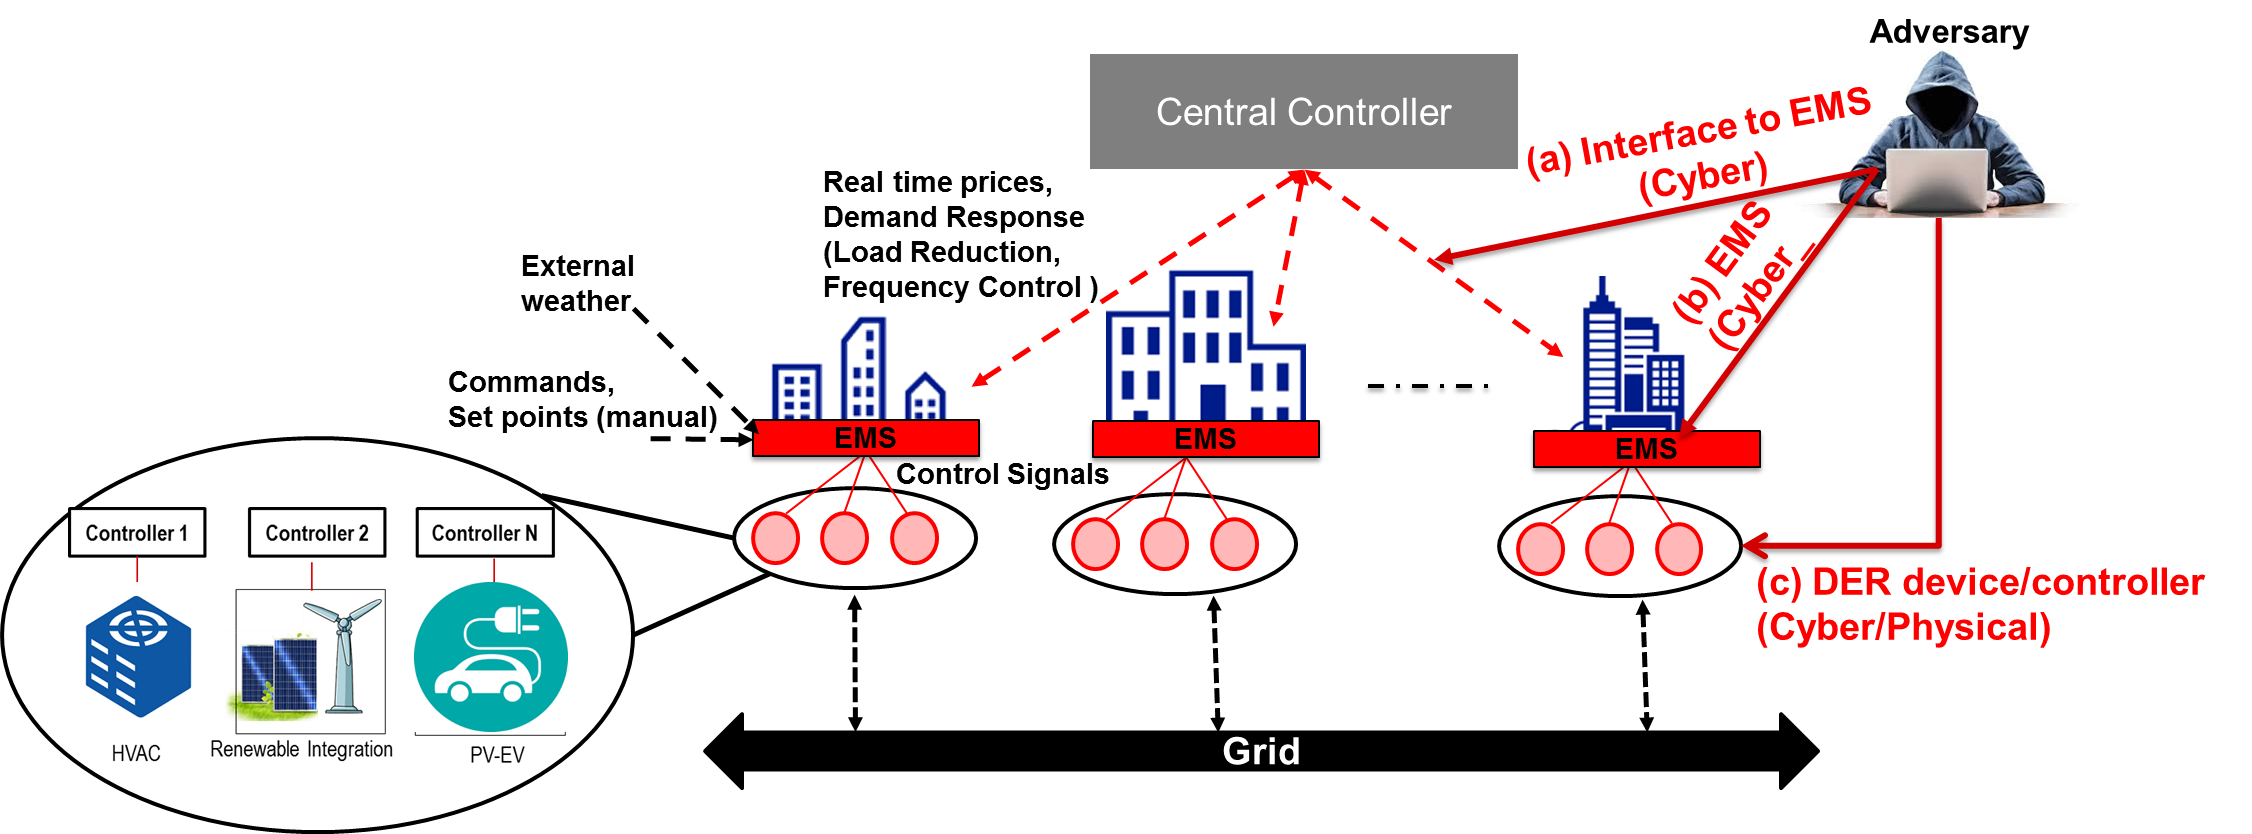
\includegraphics[width=1.1\linewidth]{figures/adversary.png}
	\caption{Adversary Model}
	\label{ad}
\end{figure}

In earlier sections, we mainly presented how an attacker can compromise the building to grid systems to lauch the attacks; in sequel, we discuss about what an attacker can perform if he gains access to the systems. Various attack scenarios in reference to NESCOR is listed below \cite{Lee:NESCOR2013}. 


\begin{itemize}
 \item Attacker issues mass remote disconnect command to DERs from the central controller 
  \item Attacker issues remote disconnect/reconnect commands in a specific order to create surge to the DERs 
 \item Attacker tampers with the DER data sent to the EMS or to the detection module to remain undetected (e.g., false data injection by exploiting the unsecured communication to compromise the input-output signals of the DER or the DER control algorithm itself)
 \item Attacker exploits invalid access control or software errors in EMS to install malware on DER device. The control algorithm and/or the input-outputs of the device are assumed to be compromised. The malware provides a way for the attacker to  remotely connect and control the devices 
 \item Attacker compromises the broadcast key that is used to communicate with the DER from the central controller (utility or main control center). The communications can be spoofed to and from the device. An attack may include a false data injection to hide the attack or underestimate or overestimate the energy consumption or production 
 \item Attacker sends unauthorized pricing information to the EMS which has the potential to create a brownout or blackout (e.g., lower pricing causes larger demand and higher pricing causes decreased demand, ultimately leading to demand supply mismatch) 
  \item Attacker sends false responses to the pricing commands from the central controller,  forcing central controller to take faulty decisions . 
 \item Attacker performs denial of service attack or out-of-sync attack on the demand response messages so that the messages are not received by EMS from the central controller on-time  
 \item Attacker gains unauthorized access to the EMS web interface and issues an invalid command to the DERs or changes the set points and other parameters of the device 
 \item Attacker reverse engineers DER devices, uses the SHODAN tool to map all vulnerable devices and issues simultaneous disconnect/reconnect commands or sends response messages that can cause electricity consumption to go high during peak times or send messages that changes the ramp rate, trip time or volt-var set points to cause voltage fluctuations 
 \item Attacker  installs a vulnerable version of the firmware and and attacker will now be able to control DER input-output or the control logic
 \item Attacker exploits access control flaws of  DERs or EMS to change the DER settings (e.g., set longer trip-off time so that the DER does not trip when voltage changes to low or high or change the active-reactive power profile) 
 \item Attacker uses the malware installed during deployment (supply chain attack) to ignore the utility messages  or change the control parameters or settings 
 \item Attacker send the wrong or compromised sequence of commands to the DER
 \item Attacker might be able to install malware on the EMS or DER that fails to respond to utility requests 
 \item Custom malware at central controller sends demand response messages that are apt for non-peak times at peak-times (addition of load at peak times and reduction of load at peak times) 
 \item Modified settings at the EMS or DER causes the device to supply erratic volt-var or other service 
\end{itemize}

\subsection{Attack Impact Analysis}
By attacking the grid-edge systems, an attacker can influence a number of system actions, as identified by \cite{DER:2017}. This ranges from voltage-frequency violations to grid instabilities.  

\begin{enumerate}
\item Disconnect: The DER can be tripped off from the grid. This can
prevent the consumer from selling back energy to the grid, and it
may also negatively influence grid operation by creating frequency
or voltage violations or influencing the system stability.

\item  False trip: If the PV manipulation can masquerade as a fault, the
attacker could potentially trigger an incorrect tripping of a protection
relay. This attack could cut off power to a number of consumers on a
distribution feeder.

\item  Overloads: Under light load conditions or when the load is
disconnected either by the operator or by an attacker, the power from PV or other DER devices can flow back to the substation and
may cause overloading of the feeder between the DER system and
the substation. If PV generation masks the actual load, the
unexpected disconnection of PV may cause overloading of the
feeder; more generally, manipulating the active power of many
DER devices can change the power flow of the distribution
system, which can cause further power flow violations~\cite{Solar}.

\item Voltage-frequency violations: Malicious control of a smart
inverter could cause a violation of acceptable grid voltage and
frequency ranges, resulting in grid instabilities, and potential
outages. High penetration of DER can influence voltage profile
and system frequency, depending on the location and capacity of
the DER and their loading conditions.

\item Failed protection: The DER operation can mask a real system
fault such that a protection device does not operate correctly,
causing a fault to propagate. Reverse power flow caused by DER
can lead to exceeding the interruption ratings of circuit protections
and sympathetic tripping of adjacent circuits~\cite{Solar}. High PV
penetration can change the fault current levels and the protection
zone of the protective relays, and may influence the coordination
of overcurrent relays, fuses, sectionalisers, and auto-reclosers~\cite{Solar}.
The misoperations of protective relays may even lead to a
cascading event in the distribution grid.

\item System instability: Manipulating the active and reactive powers of
a large number of DER can influence the small-signal stability and
voltage stability of the power system, which may cause undamped
oscillations or voltage collapse.

\end{enumerate}
\subsection{Attack Scenarios} 
\subsubsection{Demand Response}
Under a Demand Response (DR) program the consumer loads are controlled in responsive to the conditions in the electric power system, in order to achieve better efficiency of the retail market. The objective of the malicious attacker will be to damage the power grid by generating sudden overload spikes via arbitrarily sending commands (e.g., switch on/off commands) to curtail loads to consumers under Direct Load Control (DLC)~\cite{Amini:ISGT2015} or via sending arbitrary incentive price signals to consumers under dynamic pricing schemes~\cite{Liu:DSC2016}. One way to achieve this is to to block communications between
a demand response automation server and a customer
system (smart meters or customer devices) by flooding
the communications channel with other messages, or by
tampering the communications channel~\cite{Lee:NESCOR2013}. Then, the
attacker can maliciously send commands or pricing signals that can cause the maximum sudden overload in the power distribution network, which can potentially cause blackouts because of equipment failures
(e.g. burnt transformers) and circuit breakers opening. 

\textbf{Attacker objective:} Voltage-frequency violations, system overload, system instability and increased operating costs for customer 
\subsubsection{Load Switching}
Recently, researchers have shown the feasibility of attacking and destabilizing the grid by cleverly manipulating the loads from the edge and creating a relatively rapid dynamic effect~\cite{Amini:ISGT2015}. What is unique about the attack they investigated is that it can be accomplished using smart meters that are relatively easy to acquire as opposed to many attacked described in the literature that require access to more specialized power system equipment, control systems, or both (e.g., voltage regulation devices or the communication network that carries signals for load frequency control). In this attack, the attacker gains control over a substantial quantity of load simultaneously (e.g., perform mass disconnect or send fake DR messages) by hijacking a large number of smart meters~\cite{Lee:NESCOR2013}. Using these meters, the attacker creates a large imbalance between power demand and power supply by switching off the load under the attacker's control. This causes a large sudden change in the frequency of the power system, thereby forcing some generators to disconnect from it. By continuing this attack multiple times, 
%several times in the course of a few minutes, 
large number of generators can be forced to disconnect in a few minutes, thereby instigating a large-scale blackout. With the grid being modernized, clearly such attacks from end-user devices are likely to increase. 
For example, such power imbalance can be created by disconnecting or connecting the energy loads at a certain frequency through the Direct Load Control demand response program.

\textbf{Attacker objective:} System instability/unbalancing
%For e.g., attacker can exploit the Direct Load Control demand response program to disconnect and connect the loads at a certain frequency to cause the imbalance.
\subsubsection{Distributed generation}
High penetration level of photovoltaics (PV) on distribution system present several opportunities
and challenges for power distribution utilities. Major adverse impacts of high PV penetration are on system
voltages (steady state voltage rises due to reverse power flow and voltage fluctuations caused by rapid changes in the PV output). One approach to offset the voltage rise in distribution networks is to exploit the inherent reactive power capability of the PV inverters that can inject or absorb reactive power as needed. In order to rectify the fluctuations in the PV output due to the large variance of solar irradiance, ramp rate control strategies are leveraged~\cite{Alam:EC2014}. The objective of the malicious attacker is to disrupt the reactive power provided by inverters or adjust the ramp control rate to create significant voltage rises and fluctuations that may look as  normal disturbances and not cyber attack. Under light load/heavy load conditions, an attacker can issue mass connect (to the grid) or disconnect (from the house) command to PVs causing increased reverse power flow/supply-demand mismatch, respectively. 

\textbf{Attacker objective:} Voltage-frequency violations (via  creating larger fluctuations in solar power or injecting unexpected active/reactive power), system overload (via disconnect attack), system instability and equipment damage 
\subsubsection{Ancillary Services}
To guarantee high quality power supply, various ancillary services are provided by power plants to maintain the stability of power grid, such as reactive power/frequency control, voltage regulation, load following and etc. With the advent of advanced metering technologies and increasing popularity of intermittent renewable energy resources in the power grid, the distributed power generation units are playing an important role in providing ancillary services~\cite{Hess:SGT2016,Pires:IES2016,Kim:PS2017}. To make accurate decisions and maintain the reliability of power network, the utility is highly dependent on the low latency communication infrastructures to measure system states and dispatch control signals~\cite{Cleveland:2013}. This dependency can be leveraged by attackers to disrupt the stability of power network by sending fake measurements to utilities or blocking/manipulating control signals to DER devices~\cite{Srikantha:ISGT2015}. On the other hand, the attacker can also proactively obtain control over DER devices to maliciously create a power spike or inject excessive reactive power into the system.

\textbf{Attacker objective:} Voltage-frequency violations, system instability 
\subsubsection{Electric vehicles}
Electric vehicle charging has become a significant energy load in many commercial and residential buildings, and will likely continue growing rapidly due to its high power efficiency and low carbon emission~\cite{Wei:ICCAD2014}. EVs can be charged at various levels of charging rate, with increasing capacity of battery, EV charging can provide significant energy flexibility, and it is also becoming an important part of the power grid by providing different types of ancillary services~\cite{Knezovic:TE2017}, such as reactive power compensation~\cite{Buja:PE2017}, frequency regulation~\cite{Guo:ICC2016}, V2G services~\cite{Mohamed:PEC2016} and etc. Due to the wide distribution and easy access, the EV infrastructure can be the most vulnerable part of the power grid under malicious cyber attacks~\cite{Mousavian:GW2015,Ghansah:PIER2009}. Malwares can be uploaded to the EV charging station by malicious attackers, due to the high mobility of EVs, the malwares can propagate and spread rapidly, and even compromise other smart grid equipment, such as PMUs and smart meters. Then attackers can increase the power/voltage fluctuation by sending false electricity price or mislead utility operations by injecting fake power demand through the compromised smart meters and EV infrastructures~\cite{Ahmed:2016}. Furthermore, attackers can also coordinate the operation of large number of compromised EV charging stations to maliciously create a huge peak power demand and disrupt the stability of power grid and even lead to a local outage.

\textbf{Attacker objective:} Voltage-frequency violations, system overload, system instability, equipment damage 
\section{INGRESS: Integration of Green Renewable Energy Sources Securely with the Buildings and the Electric Power}
\label{sec:ingress}
Clearly, there is a strong need for the development of techniques to detect attacks launched from the grid-edge devices. We present INGRESS that is based on the development of conceptual models of the controlled grid-edge devices in an automated and non-intrusive manner by harnessing both data-driven and model based techniques on various sources of data streams that includes (i) voltage magnitude and phase angles from $\mu$PMUs; (ii)  active power and reactive power of individual devices; (iii) operating states of the devices and other auxiliary information such as weather, external data feeds etc. While the datastreams from $\mu$PMUs and devices enables INGRESS to infer the condition of the grid where the DERs are being integrated, the individual information about teh behavior of device enables INGRESS to detect abnormal behaviors and localize the attack. As shown in Figure~\ref{overview}(a), we consider a distributed agent framework where each individual INGRESS agent provides a local observation of the DER and the area where it is integrated. The local observations from INGRESS agents are sent to an INGRESS Aggregator. We consider that the distribution network is split into multiple areas, where each area is equipped with an Aggregator. The Aggregator also has access to the $\mu$PMUs and other distribution grid network information (for e.g., conditions of the switches and breakers) which facilitates distributed state estimation and other power system analysis. The information from multiple INGRESS modules and the area-based state estimation results are further used by INGRESS Aggregator to identify and localize the anomalous behaviors. On the event of detection of an anomalous behavior, INGRESS Aggregator informs the central controller. 
Figure~\ref{overview} provides a high level architecture diagram of INGRESS.
\begin{figure}[t!]
	\centering
	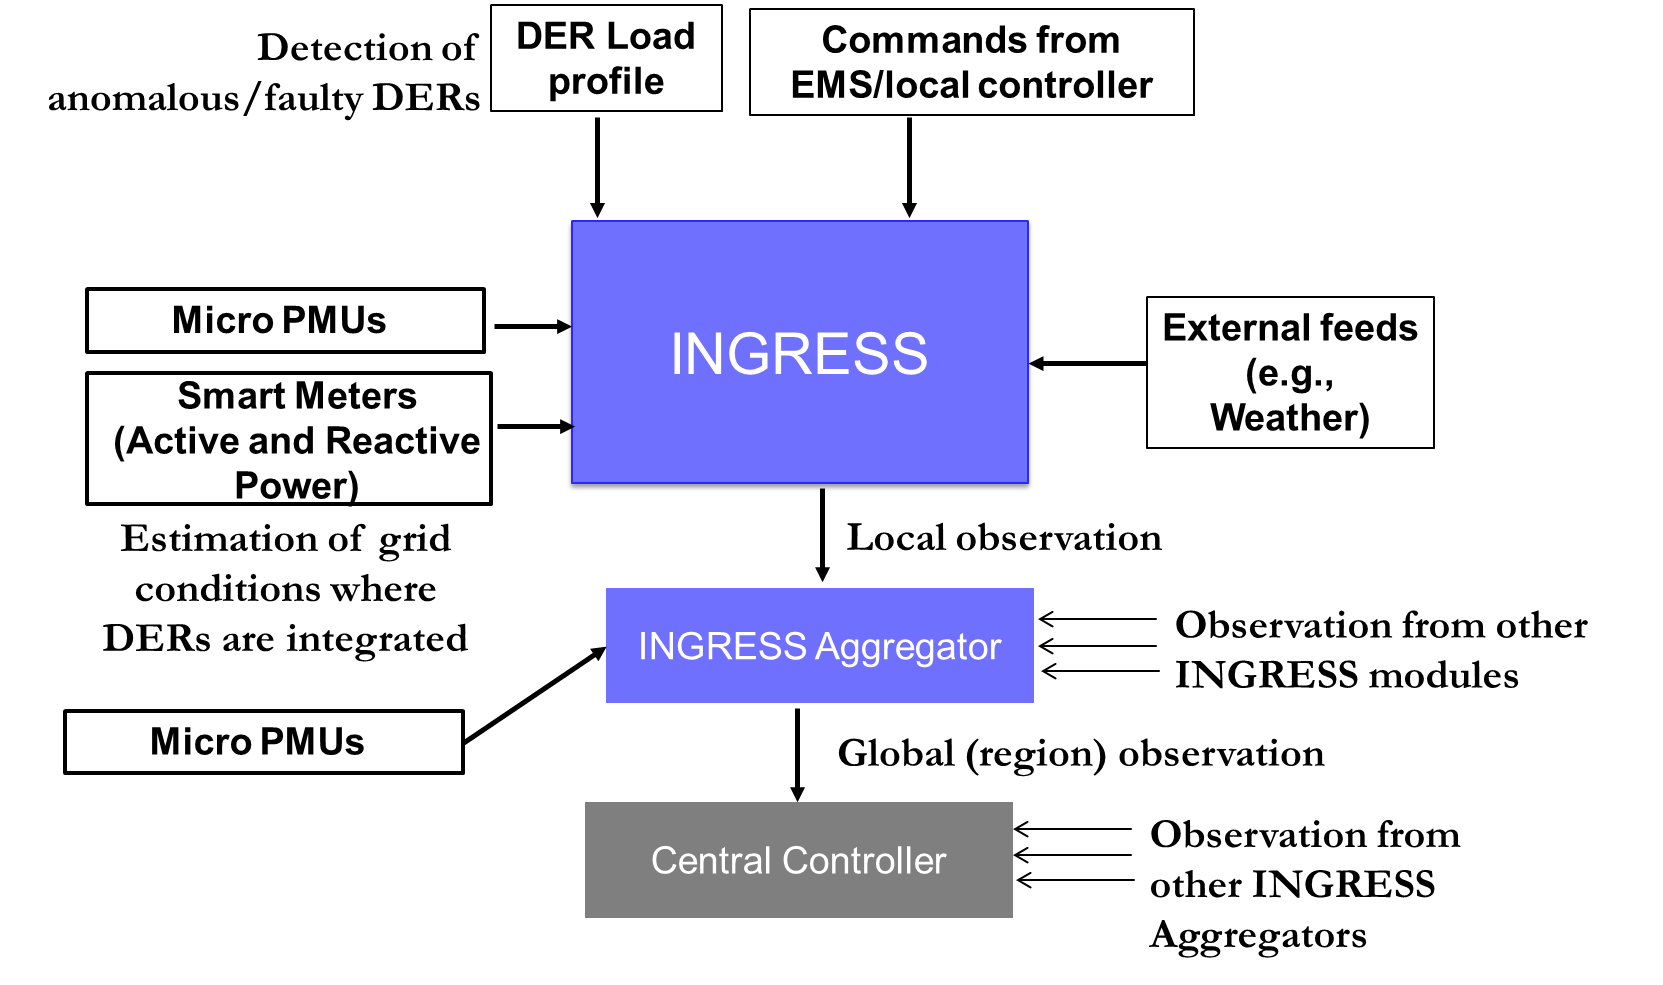
\includegraphics[width=1.1\linewidth]{figures/ingress.png}
	\caption{Datastreams and the communication architecture of INGRESS}
	\label{overview}
\end{figure}

\section{Conclusion}
\label{sec:conclusion}
In this paper, we outlined the various cyber-physical attacks that can be launched from the grid-edge systems and then presented a high level architecture design of INGRESS deployable for both  legacy and emerging behind-the-meter DERs.  INGRESS assumes a hierarchical distributed agent based framework and relies on the development of normal behavior models of the grid-edge devices in an automated and non-intrusive manner by using a combination of data-driven and model based techniques on multiple sources of information that capture the conditions of DERs and of the power system area where the DERs are integrated. The use of multiple sources of information enables INGRESS to detect anomalous behaviors with increased accuracy.

\section*{Acknowledgment}
This material is based upon work supported by the Department of Energy under Award Number(s) DE-OE0000826.
\section*{Disclaimer}
This paper was prepared as an account of work sponsored by an agency of the United States Government.  Neither the United States Government nor any agency thereof, nor any of their employees, makes any warranty, express or implied, or assumes any legal liability or responsibility for the accuracy, completeness, or usefulness of any information, apparatus, product, or process disclosed, or represents that its use would not infringe privately owned rights.  Reference herein to any specific commercial product, process, or service by trade name, trademark, manufacturer, or otherwise does not necessarily constitute or imply its endorsement, recommendation, or favoring by the United States Government or any agency thereof.  The views and opinions of authors expressed herein do not necessarily state or reflect those of the United States Government or any agency thereof.



\bibliographystyle{ieeetr}
\bibliography{references}


\end{document}
